\subsection{Rust}

Rust ist eine compilierte system Programiersprache, welche trotz high level Features hohe Ausführungsgeschwindigkeiten verspricht. Anders als herkömmliche Programiersprachen verwendet Rust keinen Garbage Compiler, jedoch garantiert sie mit ihrem unkonventionellen \ac{RAII} Borrow Checker trotzdem Memory Safety.


Rust wurde 2006 von Softwareentwickler Graydon Hoare erfunden und wird seit 2009 von Mozilla gesponsort\cite{rust_ursprung}. In den letzten jahren verwenden immer mehr Entwickler, auch große firmen wie Google, Rust für ihre Projekte. Rust ist eine der am schnellsten wachsenden Programmiersprachen und hat sich in den letzten Jahren zu einer der beliebtesten System Programmiersprachen entwickelt \cite{stackoverflow_survey}.

Rust wurde vom Projektteam für den Turm Prototypen verwendet.

\begin{figure}[H]
  \centering
  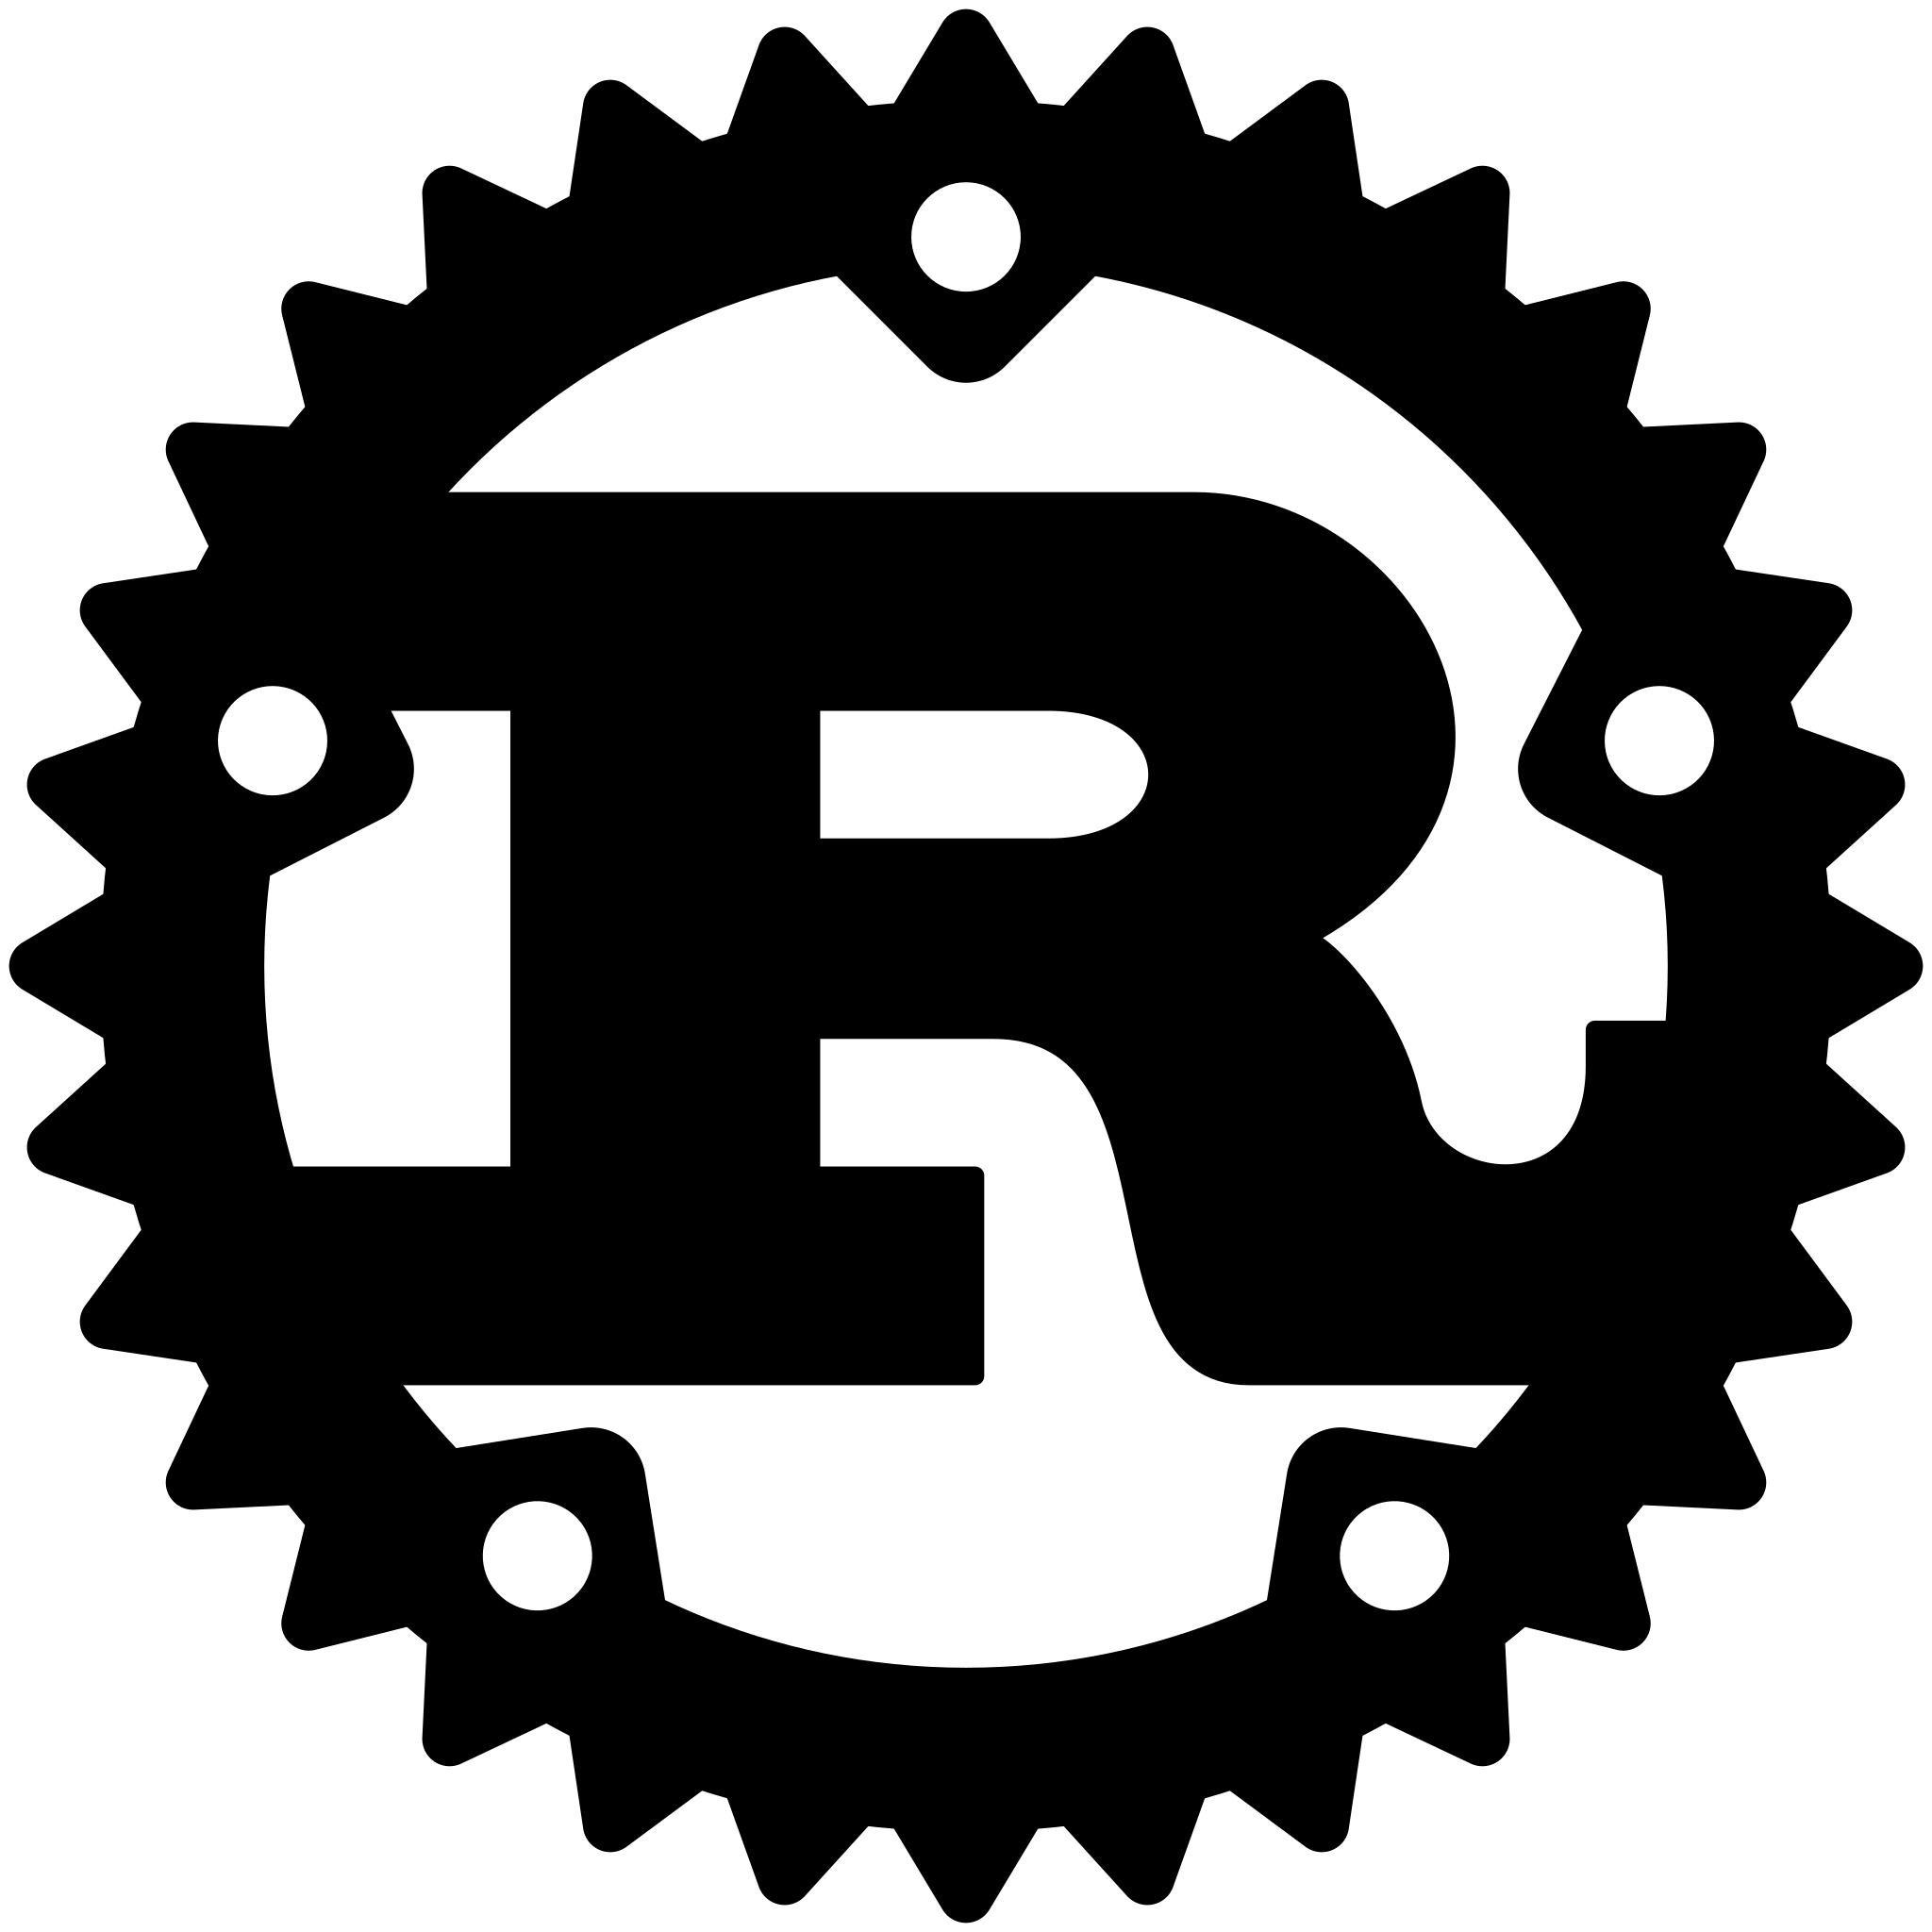
\includegraphics[width=0.20\textwidth]{images/rust_logo.png}
  \caption{Rust Logo}
  \label{fig:rust_logo}
\end{figure}

\subsubsection{\texttt{firestore\_rs} Softwarebibliothek}

Die \texttt{firestore\_rs} Softwarebibliothek ist eine Rust Softwarebibliothek, welche die Kommunikation mit der Google Firestore Datenbank vereinfacht. Die Softwarebibliothek ist Open Source auf GitHub und kann sehr einfach mittels crates.io zu einem Projekt hinzugefügt werden. Die Softwarebibliothek ist sehr einfach zu bedienen und bietet eine große Anzahl an Funktionen, welche die Kommunikation mit der Firestore Datenbank vereinfachen.

Die Bibliothek umfasst unter anderem folgende Funktionen:
\begin{itemize}
  \item \ac{CRUD} Operationen
  \item Querys erstellen
  \item Datenbank Listener
\end{itemize}

Vorallem die Listener Funktion war für das Projekt sehr wichtig, da dieses Feature zu kompliziert ist, um es selbst zu implementieren. Die Listener Funktion ermöglicht es, dass sich das System automatisch aktualisiert, wenn sich Daten in der Datenbank ändern. Dieses Feature ist für das Projekt sehr wichtig, da es die Kommunikation zwischen den einzelnen Komponenten vereinfacht.

Es wurden kleinere Änderungen an der Softwarebibliothek vorgenommen, um die Kommunikation mit der Datenbank zu vereinfachen. Die Änderungen wurden in einem Fork der Softwarebibliothek vorgenommen und können im GitHub Repository\footnote{\url{https://github.com/jokil123/firestore-rs}} eingesehen werden. Manche dieser Änderungen wurden mittels einer \Gls{pullrequest} bereits in den \Gls{masterbranch} der Softwarebibliothek übernommen und sind ab Version \texttt{v0.29.0} verfügbar.